
\documentclass[12pt]{article}

\usepackage{graphicx}
%\usepackage{subcaption}
\usepackage{amsmath}
\usepackage{amssymb}
%\usepackage{afterpage}
%\usepackage{showlabels}
% \usepackage{epstopdf}
% \usepackage{pdfpages}
\usepackage{geometry}
%\usepackage{wrapfig}
\usepackage{url}
\usepackage{times}
\usepackage{pdfpages}
\usepackage{etoolbox}
\usepackage{hyperref}
\usepackage{enumitem}
\hypersetup{
    colorlinks=true,
    linkcolor=blue,
    filecolor=magenta,
    urlcolor=cyan,
    pdftitle={Overleaf Example},
    pdfpagemode=FullScreen,
    }

\urlstyle{same}

%\usepackage{cprog}
%\usepackage[compact]{titlesec}
%\titlespacing{\section}{0pt}{5pt}{5pt}
%\titlespacing{\subsection}{0pt}{*0}{*0}
%\titlespacing{\subsubsection}{0pt}{*0}{*0}
%\usepackage[belowskip=-10pt,aboveskip=0pt,margin=10pt,font=footnotesize,labelfont=bf]{caption}

\newcommand{\shortlist}{%
\parindent 0in%
\parskip   0in%
\itemsep   0in%
\topsep    0in%
\parsep    0in%
}

\setlength{\parindent}{0in}

\geometry{letterpaper,tmargin=1in,bmargin=1in,lmargin=1in,rmargin=1in}

%\newcommand{\soln}[1] {\textit{Solution:} #1}

\newcommand{\Title}{PHYS 615 -- HW 3}

\begin{document}

\begin{center}
  {\Large\bfseries\Title}

\end{center}
\bigskip
\bigskip

\textbf{Types of homework questions}
\begin{itemize}\shortlist
  \item	RQ (Reading questions):  prompt you to go back to the text and read and think about the text more carefully and explain in your own words. While not directly tested in quizzes, can help you think more deeply about quiz questions.
  \item	BF (Building foundations):  gives you an opportunity to build and practice foundational skills that you have, presumably, seen before.
  \item	TQQ (typical quiz questions):   Similar questions (though perhaps longer or shorter) will be asked on quizzes.  But the difficulty level and skills tested will be similar.
  \item Design (D):  These are questions in which you are given a desired outcome and asked to figure out how to make it happen.  These will often also be TQQ’s, but always starting with desired motion/behavior as the given.
  \item	COMP (Computing): computing questions often related to TQQ but will never be asked on a quiz (since debugging can take so long).  You will need to do at least four computing questions over the semester
  \item	FC (free choice): allows you to decide where to put your time.  Any of the following are possible:  work through a section of the text or a lecture in detail; redo a problem from before; do an unassigned problem in the text; extend a computing project; try a problem using a different analytical approach (e.g. forces instead of conservation of energy).
  \item ACT (in-class activity): These questions are repeats of questions (or similar to) that occurred in a previous in-class activity.
  \item \textbf{Standard Reading Questions}: How does the reading connect with what you already know? What was something new?  Ask an "I wonder" question OR give an example applying the idea in the reading.
\end{itemize}

\textbf{Please remember to say something about the "Check/Learn" part at the end of solving a problem!}

Note that while this homework does not have designated "RQ" questions, in particular the activity-based questions can certainly benefit from reading the corresponding sections in the text.

Full credit will be given at 75\% of the total points possible, so you can choose a subset of problems (you can do more / all, but the score is capped at 75\%)

\begin{enumerate}
  \item COMP (10 points) Now that you have, presumably, a working numerical solver for the skateboard problem, there's actually no need to use the small angle approximation anymore -- we can instead solve the full problem with very  little additional work:
        \begin{align}
          \ddot \phi = -\frac{g}{R} \sin \phi
        \end{align}

        Change your code to solve the original ODE, and compare results. Try some different initial conditions and determine experimentally (ie., on the computer), where the small-angle approximation is a good approximation, and when it leads to noticable deviations. As you have seen in last week's problem, the Euler method generates errors of its own, which can be kept under control by making the timestep pretty small, so be sure to do so.

        \soln{See \url{https://github.com/germasch/hw/blob/main/notebooks/hw3-skateboard.ipynb} (Note: Sometimes github has issues displaying Jupyter notebooks. In that case, reload the page and it usually works the 2nd time around.)}

  \item TQQ / ACT (20 points) (This was activity 1.4 -- if you have your work from it, you can hand it in as-is, you don't need to write things down again.)

        \textbf{Air resistance and Newton's 2nd Law.} Suppose that you took a small rubber ball to the top of a very tall building and dropped it from rest at $t = 0$. At a later time, the ball moves with \textit{constant speed}. (That speed is called \textit{terminal speed}.)

        \soln{See the solution to activity 1.4.}

        \begin{enumerate}
          \item

                Draw separate free body diagrams for the ball (i) at time $t = 0$, and (ii) after it has reached terminal speed. Clearly label all forces.

          \item
                What can be said about the acceleration of the ball (i) at time $t = 0$, and (ii) after it has reached terminal speed. Discuss both magnitude and direction. How are your answers related to the FBDs above?

          \item Sketch a qualitatively correct graph of velocity vs time for the ball. Since the ball is falling down, let's take the down direction to be positive.

          \item
                On the same graph, show the $v$ vs $t$ graph for the case of no air resistance. Make sure it is otherwise consistent with the first graph you drew.

        \end{enumerate}

        \textbf{Calculating terminal speed}

        \begin{enumerate}[resume]
          \item Let's still keep downward to be the positive direction.

                Starting with Newton's 2nd Law, write an equation that includes the acceleration $\dot v$ of the ball and all relevant force terms ($mg$, linear drag $bv$, quadratic drag $cv^2$ -- see Taylor 2.1).

          \item How would your equation be different if the ball was instead moving upward?

          \item Back to dropping the ball: If the force of air resistance were purely linear with respect to velocity (ie., $b \ne 0, c = 0$), use the appropriate equation to express the terminal speed $v_t$ of the object in terms of $b$, $m$ and $g$.

                Check that your expression for $v_t$ has the correct units. That is, determine the appropriate units for $b$ and confirm that your expression for $v_t$ does have the appropriate units for a speed.
        \end{enumerate}

  \item TQQ / ACT (20 points) (This was activity 2.1 Question 2. I varied the last part of it, though)

        We're still considering motion when linear drag is present. Let $y$ be the vertical direction, positive pointing downward (that's what the text chose). In the vertical direction, since we live on Earth, we better take into account gravity, so we now have two forces $\vec F_{D,lin}$, and also $\vec F_G = mg \hat y$.

        \begin{enumerate}
          \item Write down Newton's Law in the $y$ direction and show that you get the equation
                \begin{align}
                  \dot v_y + \frac{1}{\tau} v_y = g
                \end{align}

                \soln{
                  \begin{align*}
                    m \dot v_y & = mg - b v_y          \\
                    \dot v_y   & = g - \frac{b}{m} v_y
                  \end{align*}
                  Which can be written in the given form by defining $\tau = \frac{m}{b}$.
                }

          \item You had already derived terminal speed $v_{ter} = \frac{mg}{b}$ in a previous activity (ie., above). Show that you get the same answer from the differential equation for $v_y$ under the assumption that the terminal speed is the \textit{constant} speed that gets reached eventually.

                \soln{
                  \begin{align*}
                    \dot v_y + \frac{1}{\tau} v_y & = g                    \\
                    \frac{1}{\tau} v_{ter}        & = g                    \\
                    v_{ter}                       & = g\tau = \frac{mg}{b}
                  \end{align*}
                  Which is the same answer.
                }

          \item It makes some sense to express our ODE in terms of $v_{ter}$. Solve the equation for $v_{ter}$ for $g$ and plug that expression into the ODE above. Show that you end up with
                \begin{align}
                  \dot v_y + \frac{1}{\tau} v_y = \frac{1}{\tau} v_{ter}
                \end{align}

                \soln{Solving for $g$ gives $g = v_{ter}{\tau}$, and that just needs to be plugged in to get the desired answer.}
        \end{enumerate}

        We now have an inhomogeneous (a.k.a. non-homogeneous) ODE to solve. We could do this by finding a particular solution and adding the set of homogeneous solutions, but let's practice another way.

        \begin{enumerate}[resume]

          \item Introduce a new variable $u = v_y - v_{ter}$. Rewrite the ODE above in terms of $u$. (In order to do so, find $v_y$ in terms of $u$, and also find $\dot v_y$ in terms of $u$ and substitute those in.)

                \soln{
                  Solving the $u$ equation for $v_y$ gives $v_y(t) = u(t) + v_{ter}$, where I temporarily added $(t)$ to make explicit what quantities depend on time.

                  Taking the time derivative: $\dot v_y = \dot u + 0$. Finally, plugging those in:
                  \begin{align*}
                    \dot v_y + \frac{1}{\tau} v_y         & = \frac{1}{\tau} v_{ter} \\
                    \dot u + \frac{1}{\tau} (u + v_{ter}) & = \frac{1}{\tau} v_{ter} \\
                    \dot u + \frac{1}{\tau} u             & = 0
                  \end{align*}
                }

          \item The differential equation for $u$ should look familiar. Solve it. (It can be solved by separation of variables, but you can also just write down the solution if you know it, and verify that it is in fact a solution.) Make sure it is the general solution, ie., it should have one constant of integration, since it's a 1st order ODE.

                \soln{Let's do separation of variables, because -- why not\dots
                  \begin{align*}
                    \frac{du}{dt}                & = - \frac{1}{\tau} u           \\
                    \frac{du}{u}                 & = -\frac{1}{\tau} dt           \\
                    \int_{u_0}^u \frac{du'}{u'}  & = -\frac{1}{\tau} \int_0^t dt' \\
                    \left. \ln u'\right|_{u_0}^u & = -\frac{1}{\tau} t'|_0^t      \\
                    \ln \frac{u}{u_0}            & = -\frac{t}{\tau}              \\
                    u                            & = u_0 e^{-t/\tau}
                  \end{align*}
                }
          \item Now recast your solution in terms of $v_y$, ie., undo your substitution.

                \soln{
                  $$ v_y = u + v_{ter} = u_0 e^{-t/\tau} + v_{ter} = (v_{0y} - v_{ter}) e^{-t/\tau} + v_{ter}$$
                }


          \item Let's call our initial velocity $v_y(0) = v_{0y}$. Find the constant of integration given that condition, and rewrite the solution in terms of $v_{0y}$.

                \soln{By choosing to using definite integrals, I automatically incorporated the correct constant of integration already. Doesn't hurt to check: $v_y(t=0)$ does indeed come out to be $v_{0y}$.}

          \item Integrate to find an expression for the vertical position $y(t)$.

                \soln{
                  \begin{align*}
                    y(t) & = \int v_y\,dt                                                 \\
                         & = \int \left((v_{0y} - v_{ter}) e^{-t/\tau} + v_{ter}\right)dt \\
                         & = -\tau  (v_{0y} - v_{ter}) e^{-t/\tau} + v_{ter} t + C
                  \end{align*}
                  We should determine the constant of integration, too. I'll do so by using an initial condition $y(0) = 0$, since I can always my coordinate system origin to be the starting position. (Also, it'd be quite trivial to add a $y_0$ in the end if one doesn't want to move the coordinate system.)
                  \begin{align*}
                    0                 & = y(0)                         \\
                                      & = -\tau  (v_{0y} - v_{ter})+ C \\
                    \Longrightarrow C & = \tau  (v_{0y} - v_{ter})
                  \end{align*}
                  Plugging this back in:
                  \begin{align*}
                    y(t) & = -\tau  (v_{0y} - v_{ter}) e^{-t/\tau} + v_{ter} t + \tau  (v_{0y} - v_{ter}) \\
                         & = \tau  (v_{0y} - v_{ter}) \left( 1- e^{-t/\tau}\right) + v_{ter} t
                  \end{align*}
                }

          \item Sketch $v_y(t)$ and $y(t)$.

                \soln{ ($\tau = 1$)

                  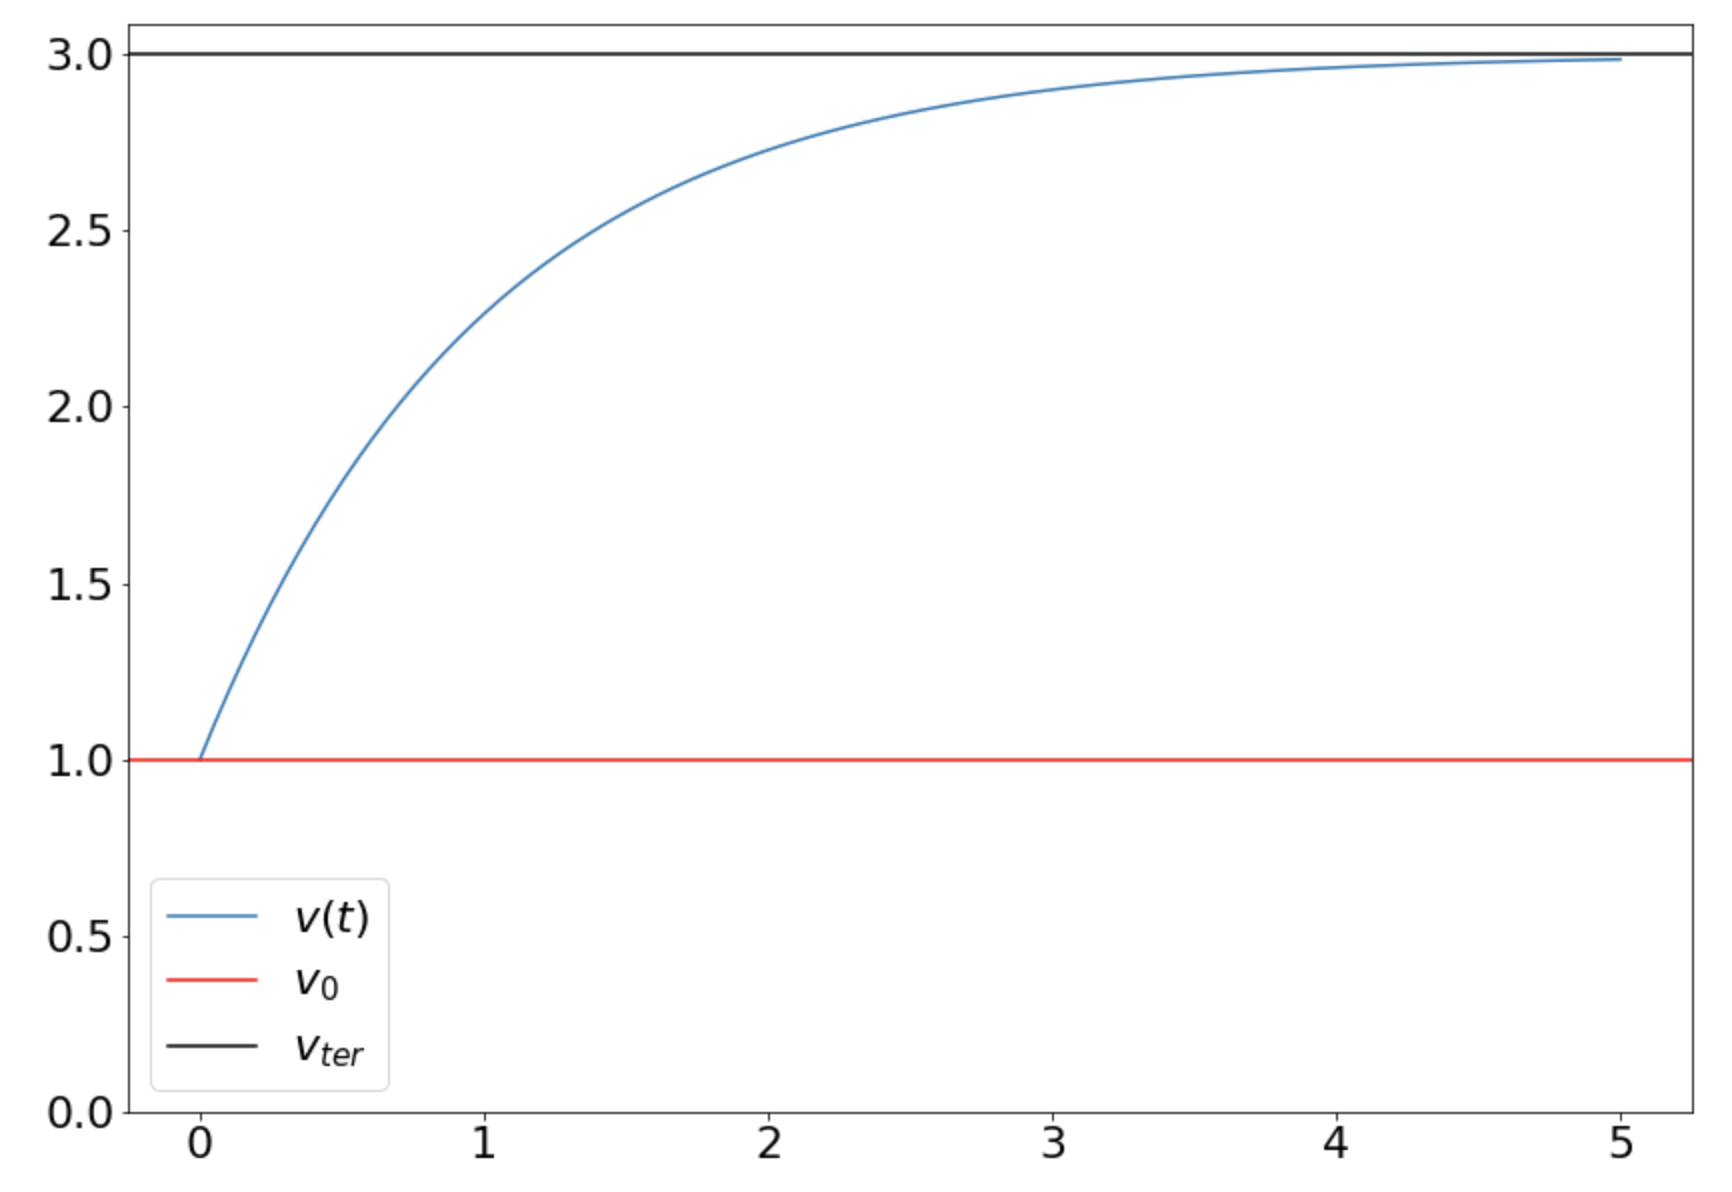
\includegraphics[width=.4\textwidth]{hw3_4.png}
                  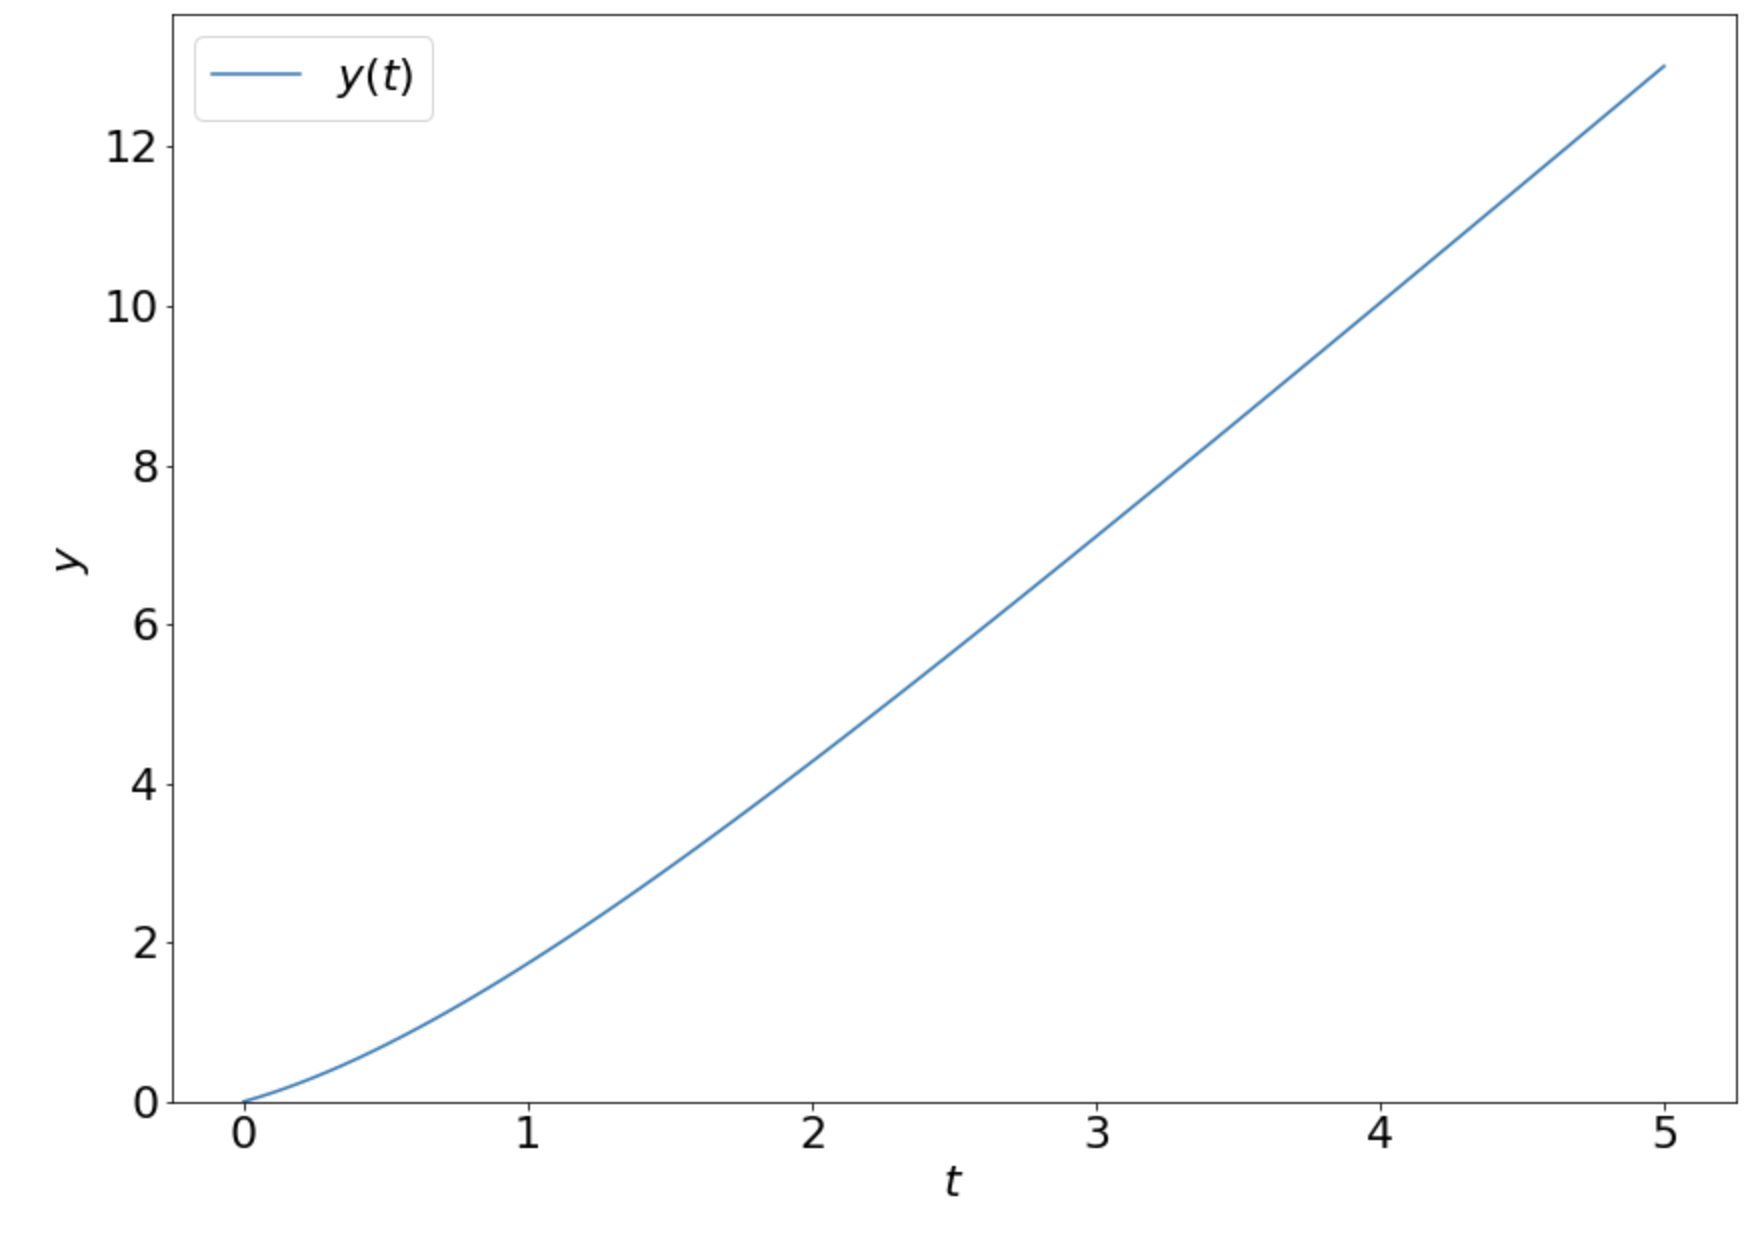
\includegraphics[width=.4\textwidth]{hw3_5.png}

                }
        \end{enumerate}

  \item TQQ / ACT (10 points)

        Find the Taylor expansion for $\ln(1-\epsilon)$ up to the cubic term in $\epsilon$. (\textbf{Show your work!})

        \soln{
          We'll need the derivatives of $\ln$:
          \begin{align*}
            \frac{d}{dx} \ln x     & = \frac{1}{x}              \\
            \frac{d^2}{dx^2} \ln x & = \frac{-1}{x^2}           \\
            \frac{d^3}{dx^3} \ln x & = \frac{(-1)(-2)}{x^3}     \\
            \frac{d^4}{dx^4} \ln x & = \frac{(-1)(-2)(-3)}{x^4} \\
          \end{align*}
          (I did one more just for fun..)

          We'll plug in $x = 1$ into those derivatives and are all set to write the Taylor expansion:
          \begin{align*}
            \ln(1-\epsilon) & \approx \ln 1 + (- \epsilon)1 + \frac{1}{2!}(-\epsilon)^2(-1) + \frac{1}{3!}(-\epsilon)^3(2)
            + \frac{1}{4!}(-\epsilon)^4(6) + \ldots                                                                           \\
                            & \approx -\epsilon - \frac{\epsilon^2}{2} - \frac{\epsilon^3}{3} - \frac{\epsilon^4}{4} - \ldots
          \end{align*}
        }

  \item TQQ / ACT (10 points) (This is the last part of activity 2.2.  -- You could use the 1st part of that activity as free-choice problem)

        Having done motion with linear drag in both the $x$ and $y$ direction in class / in the text, we can now combine these to look at projectile motion, where the objects is shot at some arbitrary angle.

        We have found two equations for $x(t)$, $y(t)$:
        \begin{align}
          x(t) & = v_{0x} \tau \left(1 - e^{-t/\tau}\right)                         \\
          y(t) & = (v_{0y} + v_{ter}) \tau \left(1 - e^{-t/\tau}\right) - v_{ter} t
        \end{align}

        where $\tau = m / b$ and $v_{ter} = \tau g$

        \begin{enumerate}
          \item We want to eliminate time to find an equation for the trajectory in the form $y(x)$. In order to do so, solve the $x(t)$ equation for time $t$, and plug that expression for $t$ into the $y(t)$ equation. Show that you get Taylor's equation (2.37):

                \begin{align}
                  y(x) = \frac{v_{0y} + v_{ter}}{v_{0x}} x + v_{ter}\tau\ln\left(1-\frac{x}{v_{0x}\tau}\right)
                \end{align}
        \end{enumerate}

        In the limit that drag is small, ie., $\frac{x}{v_{0x}\tau} \ll 1$ (why?), one would hope to get a trajectory that's close to the case without drag. Let's try that.

        \soln{$v_{0x}\tau$ is what we earlier called $x_\infty$, ie., the distance by which the drag makes the object stop. So clearly, if we're anywhere near that distance, drag has had a lot of effect. On the other hand, if we're still far away from it, ie., $x \ll v_{0x}\tau$, drag hasn't done much yet.}

        Use the Taylor expansion for $\ln(1-\epsilon)$ up to the \textit{quadratic} term to approximate the $\ln$ in your trajectory formula and compare that to the trajectory of projectile motion without drag
        \begin{align}
          y(x) = -\frac{g}{2v_{0x}^2} x^2 + \frac{v_{0y}}{v_{0x}} x
        \end{align}

        (If you didn't derive the Taylor expansion, in the previous problem, you'll need to look it up.)

        \soln{
          \begin{align}
            y(x) & = \frac{v_{0y} + v_{ter}}{v_{0x}}x + v_{ter}\tau \ln\left(1 - \frac{x}{v_{0x}\tau}\right)                                                    \\
                 & \approx \frac{v_{0y} - v_{ter}}{v_{0x}}x + v_{ter}\tau \left[ \frac{x}{v_{0x}\tau} + \frac{1}{2}\left(\frac{x}{v_{0x}\tau}\right)^2  \right] \\
                 & = \frac{v_{0y} - v_{ter}}{v_{0x}}x + \frac{v_{ter}}{v_{0x}} x - \frac{v_{ter}}{2v_{0x}^2\tau}x^2                                             \\
                 & = \frac{v_{0y}}{v_{0x}}x - \frac{v_{ter}}{2v_{0x}^2\tau}x^2                                                                                  \\
                 & = \frac{v_{0y}}{v_{0x}}x - \frac{g}{2v_{0x}^2}x^2
          \end{align}
          In the last step, I used $v_{ter} = g\tau$, and we did in fact end up with the same trajectory as in vacuum (no drag).
        }


  \item TQQ (10 points) Consider a ball moving straight upward and subject to both gravity and quadratic drag. Imagine the ball is thrown straight upward by a person on top of a tall building -- they reach their hand over the side of the building, so the ball doesn't hit the building when it comes back down. Assume that it reaches terminal velocity before hitting the ground.

        \begin{enumerate}
          \item Draw free body diagrams for both the upward and downward motion and write out Newton's 2nd Law for each case.

                \soln{

                  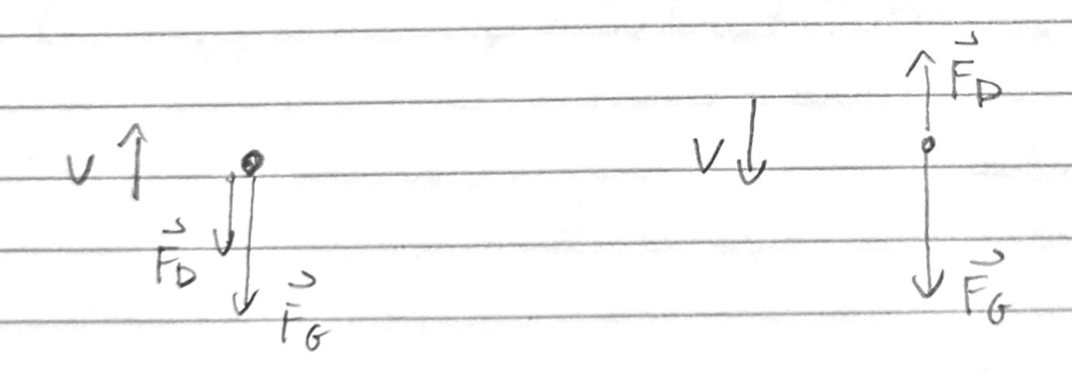
\includegraphics[width=.5\textwidth]{hw3_3.png}
                }

          \item Sketch velocity over time qualitatively.

                \soln{

                  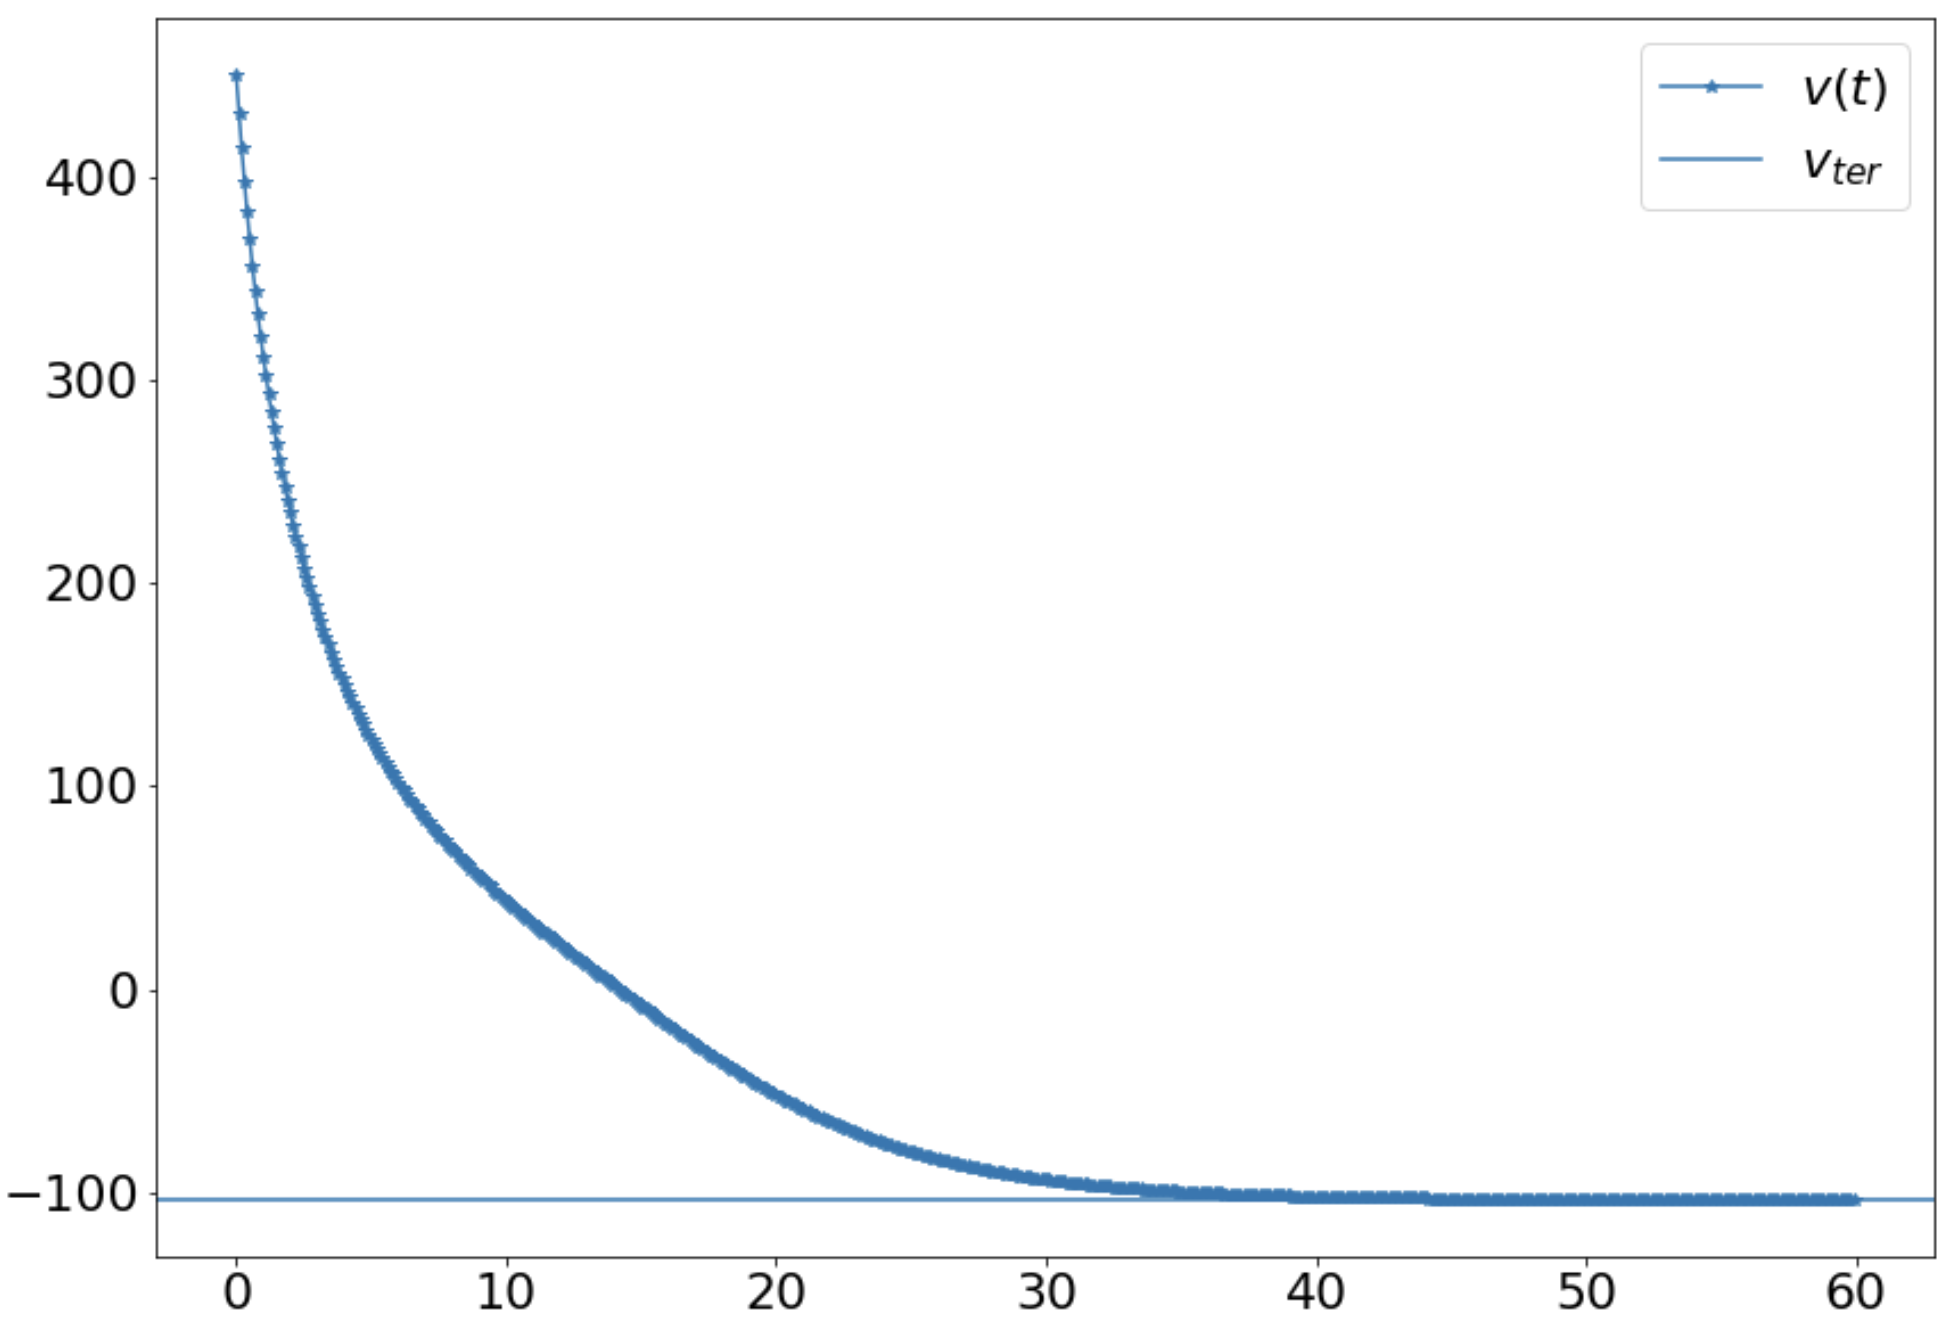
\includegraphics[width=.5\textwidth]{qdrag_up.png}}

          \item Is there a terminal velocity going upward?

                \soln{No, as can be seen from the FBD, the forces point the same direction, so they'll never cancel.}

        \end{enumerate}

  \item TQQ (10 points)

        We have found the solution for the skateboard in the half pipe to be (in the small angle approximation):
        \begin{align}
          \phi(t) = A \cos \omega_0 t + B \sin \omega_0 t
        \end{align}

        Evaluate the constants $A$, $B$ given an initial angle at time 0 of $\phi_{init}$, and an initial angular velocity for the skateboard of $\omega_{init}$.

          [Usually, we'd call these $\phi_0$ and $\omega_0$ since they're at time 0. But that would cause confusion with $\omega_0 = \sqrt{g/L}$.]

        \soln{

          Let's start by finding $\omega = \dot \phi$:
          $$\omega(t) = \dot\phi = - A\omega_0 \sin \omega_0 t + B \omega_0 \cos \omega_0 t$$

          We have two initial conditions (ie., equations), and two unknowns $A$, $B$, so things should work out, and in fact they do quite easily:

          \begin{align*}
            \phi_{init}   & = \phi(0) = A                                                             \\
            \omega_{init} & = \omega(0) = B\omega_0 \qquad \Longrightarrow B = \omega_{init}/\omega_0
          \end{align*}

          So we can rewrite the general solution as
          $$
            \phi(t) = \phi_{init} \cos \omega_0 t + \frac{\omega_{init}}{\omega_0} \sin \omega_0 t
          $$
        }





        % \item TQQ (10 points) Solve the separable differential equation
        % $$
        % \frac{dv}{dt} = a - bv
        % $$

        % where $a$ and $b$ are constants. Take the velocity at $t=0$ to be $v_0$.  Once you have that solution, find $y(t)$ given
        % $$\frac{dy}{dt} = v(t)$$

        % Be sure to plug in your functional form for $v(t)$ that you got from the first part of this problem.  Also, take $y(0)=y_0$.


  \item	FC (10 points) (free choice): allows you to decide where to put your time.  Any of the following are possible: work through a section of the text or a lecture in detail; polish up a group work assignment from class; redo a problem from before; do an unassigned problem in the text; extend a computing project; try a problem using a different analytical approach (e.g. forces instead of conservation of energy).


\end{enumerate}

\end{document}
